\documentclass[french,11pt,twoside]{article}

%%%%%%%%%%%%%%%%%%%%%%%%%%%%%%%%%%%%%%%%%%%%%%%%%%%%%%%%%%%%%%%%%%%%%%%%%%%%%%%%%%%%%%

\usepackage[utf8]{inputenc}

\usepackage{amsmath}
\usepackage{amstext}
\usepackage{amssymb}
\usepackage{graphicx}

\usepackage{url}
\usepackage[breaklinks=true]{hyperref}

\usepackage[top=2.5cm,bottom=2.5cm,right=2.5cm,left=2.5cm]{geometry}

\usepackage[francais]{babel}
\usepackage[babel=true]{csquotes}

\usepackage{listings}

\lstdefinelanguage{lsd12}{
  morekeywords={true, false, min, max, &&, ||, !, =, <, >, in, +, -, /, *, \# ,  (, ), if, hen, else, fi, while, do, od, write, read, add, to, remove, from, return, int, bool, iset, var, forward, begin, end, :, ;, program, function, void },
  string=[b]
}

\lstdefinelanguage{pcode}{
  morekeywords={lod, lda, ldc, ind, add, sto, div, mul, sub, neg, les, leq, grt, geq, equ, and, or, not, define, ujp, fjp, ssp, new, stp, mst, retp, retf },
  string=[b]
}

%%%%%%%%%%%%%%%%%%%%%%%%%%%%%%%%%%%%%%%%%%%%%%%%%%%%%%%%%%%%%%%%%%%%%%%%%%%%%%%%%%%%%%


\newcommand{\LSD}{$LSD^{{12}}$}
\newcommand{\lsd}{\LSD}


\newcommand{\terminal}[1]{\ \ensuremath{\pmb{\mathtt{#1}}\ }}
\newcommand{\nonterminal}[1]{\ \mathit{#1}\ }
\newcommand{\catsynt}[1]{\mathsf{#1}}
\newcommand{\domaine}[1]{\ {\mathbb#1} \ } 
\newcommand{\semelt}[1]{\ \mathrm{#1} \ }

                                %
                                % Crochets pour entourer les �l�ments syntaxiques.
                                %
\newcommand{\sem}{\ensuremath{[\![}}
\newcommand{\mes}{\ensuremath{]\!]}}
                                %
                                % Fonctions s�mantiques
                                %
\newcommand{\SemNum}{\ensuremath{\mathcal{N}}} %semantics of numbers
\newcommand{\SemEB}{\ensuremath{\mathcal{B}}} %semantics of boolean expressions
\newcommand{\SemED}{\ensuremath{\mathcal{E}}} %semantics of right hand-side expressions
\newcommand{\SemEG}{\ensuremath{\mathcal{A}}} %semantics of left hand-side expressions
\newcommand{\SemEE}{\ensuremath{{\mathcal{I}}}} %semantics of an integer expression
\newcommand{\SemDV}{\ensuremath{{\mathcal{D}_v}}} %semantics of a variable declaration
\newcommand{\SemDVL}{\ensuremath{{\mathcal{D}_{vl}}}} %semantics of a list of variable declarations
\newcommand{\SemDA}{\ensuremath{{\mathcal{D}_{arg}}}} %semantics of parameters
\newcommand{\SemDPL}{\ensuremath{{\mathcal{D}_{pl}}}} %semantics of a list of a procedure declaration
\newcommand{\SemDP}{\ensuremath{{\mathcal{D}_p}}} %semantics of a procedure declaration
\newcommand{\SemProg}{\ensuremath{\mathcal{P}}} %semantics of a program
\newcommand{\SemVR}{\ensuremath{{\mathcal{V}}}} %semantics of a variable reference
\newcommand{\SemI}{\ensuremath{\mathcal{S}}} %semantics of a statement
\newcommand{\SemIL}{\ensuremath{\mathcal{S}}} %semantics of a list of statements
\newcommand{\SemPar}{\ensuremath{\mathcal{P}{\textrm \it ar}}} %signature of formal parameters list
\newcommand{\SemBloc}{\ensuremath{\mathcal{B}{\textrm \it loc}}} %semantics of a bloc (declvar+declproc+instr)
\newcommand{\SemType}{\ensuremath{\mathcal{T}{\textrm{\it\!\!ype}}}} %Type of an expression
\newcommand{\SemTypeG}{\ensuremath{\mathcal{T}{\textrm{\it\!\!ype}}_G}} 
\newcommand{\SemTypeV}{\ensuremath{\mathcal{T}{\textrm{\it\!\!ype}}_V}}
\newcommand{\SemTypeF}{\ensuremath{\mathcal{T}{\textrm{\it\!\!ype}}_F}}  
\newcommand{\SemSig}{\ensuremath{\mathcal{S}{\textrm{\it\!ig}}}} 
\newcommand{\Uninit}{\textrm{uninit}}
\newcommand{\SemAlloc}{\ensuremath{\mathcal{A}{\textrm{\it\!lloc}}}}
\newcommand{\SemFun}{\ensuremath{\mathcal{F}}}
\newcommand{\SemPile}{\ensuremath{\mathcal{P}{\textrm{\it\!ile}}}}
\newcommand{\SemDAlias}{\ensuremath{{\mathcal{D}_{alias}}}}
\newcommand{\SemDAL}{\ensuremath{{\mathcal{D}_{al}}}}
\newcommand{\SemDF}{\ensuremath{{\mathcal{D}_f}}} %semantics of a function declaration
\newcommand{\SemDFL}{\ensuremath{{\mathcal{D}_{fl}}}}


%%%%%%%%%%%%%%%%%%%%%%%%%%%%%%%%%%%%%%%%%%%%%%%%%%%%%%%%%%%%%%%%%%%%%%%%%%%%%%%%%%%%%%

\title{GPMachine : Guide d'utilisation\thanks{Ce document a été élaboré en partie à partir des notes de Hubert Toussaint.}}
\author{Xavier Devroey}
\date{[INFOB314/IHDCB332] Théorie des langages : Syntaxe et sémantique}

%%%%%%%%%%%%%%%%%%%%%%%%%%%%%%%%%%%%%%%%%%%%%%%%%%%%%%%%%%%%%%%%%%%%%%%%%%%%%%%%%%%%%%
\begin{document}

\maketitle

\tableofcontents
\vspace{1cm}
\hrule

%%%%%%%%%%%%%%%%%%%%%%%%%%%%%%%%%%%%%%%%%%%%%%%%%%%%%
\section{Introduction}
%%%%%%%%%%%%%%%%%%%%%%%%%%%%%%%%%%%%%%%%%%%%%%%%%%%%%

\begin{figure}[h]
\centering
	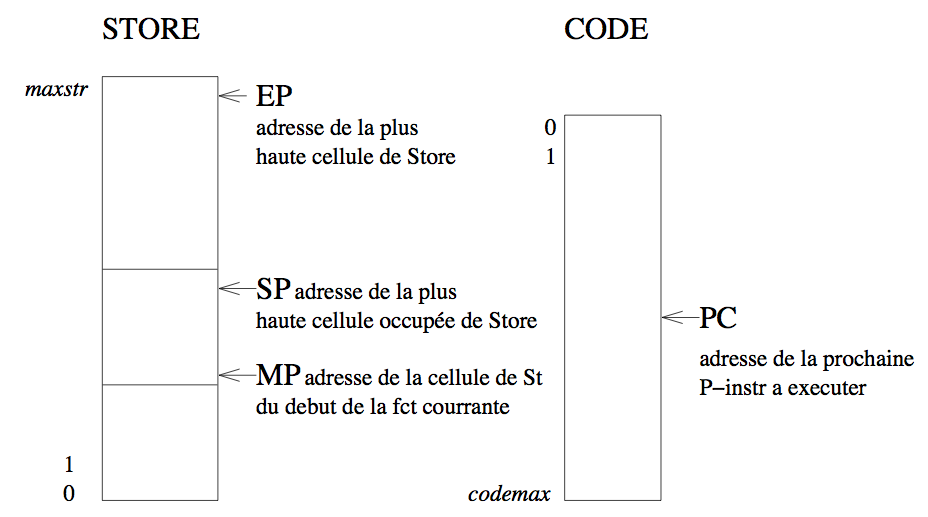
\includegraphics[width=0.8\textwidth]{images/structure-PMachine}
	\caption{Structure de la GPMachine}
	\label{fig_structure_gpmachine}
\end{figure}

La GPMachine possède
\begin{itemize}
\item une mémoire de données $STORE$ de longueur $maxstr+1$
\item une mémoire pour les P-instructions de longueur $codemax+1$
\item un registre $SP$ : contient l'adresse de la plus haute cellule occupée de $STORE$
\item un registre $EP$ : contient l'adresse de la plus haute cellule de $STORE$
\item un registre $PC$ : contient l'adresse de la prochaine P-instruction à exécuter de $CODE$
\item un registre $MP$ : contient l'adresse de la cellule de $STORE$ qui correspond au début du bloc d'activation de la fonction courante
\end{itemize}


Manipule
\begin{itemize}
\item entier ("i"), réel ("r"), booléen ("b"), adresse ("a")
\item "N" représente un type numérique : $N\in\{i,a\}$
\item "S" représente un type scalaire : $S\in\{i,b\}$
\item "T" représente un type quelconque : $T\in\{i,a,b\}$
\end{itemize}

Remarques
\begin{itemize}
\item P-Code créé pour la traduction de Pascal
\item \lsd utilise une petite partie de P-Code
\item on ne présente que la partie de P-Code nécessaire à la traduction de \lsd
\item quelques différences existent entre l'implémentation de la P-Machine qui vous est fournie et la définition qui est donnée dans WilHelm et Maurer (registre EP,instruction define,...)
\end{itemize}


%%%%%%%%%%%%%%%%%%%%%%%%%%%%%%%%%%%%%%%%%%%%%%%%%%%%%
\section{Instructions}
%%%%%%%%%%%%%%%%%%%%%%%%%%%%%%%%%%%%%%%%%%%%%%%%%%%%%


\subsection{P-Instructions pour les expressions}
%%%%%%%%%%%%%%%%%%%%%%%%%%%%%%%%%%%%%%%%%

\subsubsection{Expressions numériques}
%----------------------------------

\begin{tabular}{|l|l|c|c|}
\hline
P-Instruction     & Signification                                                              & Condition & Résultat \\
\hline
add N                & STORE[SP-1] $:=$ STORE[SP-1] $+_N$ STORE[SP];    & (N,N)        & (N)\\
                         & SP $:=$ SP $-$ 1                                                      &                 & \\
sub N                & STORE[SP-1] := STORE[SP-1] $-_N$ STORE[SP];        & (N,N)         & (N)\\
                         & SP $:=$ SP $-$ 1                                                      &                 & \\
mul N                & STORE[SP-1] := STORE[SP-1] $*_N$ STORE[SP];        & (N,N)         & (N)\\
                         & SP $:=$ SP $-$ 1                                                      &                 & \\
div N                & STORE[SP-1] := STORE[SP-1] $/_N$ STORE[SP];        & (N,N)         & (N)\\
                         & SP $:=$ SP $-$ 1                                                      &                 & \\
neg N                & STORE[SP] $:=$ $-_N$ STORE[SP]                             & (N)            & (N)\\
\hline
\end{tabular}
\\

O\`{u}  (N,N) indique que STORE[SP] et STORE[SP-1] sont de type numérique.


\subsubsection{Expressions booléennes}
%----------------------------------

\begin{tabular}{|l|l|c|c|}
\hline
P-Instruction     & Signification                                                              & Condition & Résultat \\
\hline
or b                   & STORE[SP-1] $:=$ STORE[SP-1] $or$ STORE[SP];      & (b,b)          & (b)\\
                         & SP $:=$ SP $-$ 1                                                      &                  & \\
and b                & STORE[SP-1] $:=$ STORE[SP-1] $and$ STORE[SP];    & (b,b)          & (b)\\
                         & SP $:=$ SP $-$ 1                                                      &                  & \\
not b                 & STORE[SP] $:=$ $not$ STORE[SP]                              & (b)             & (b)\\
\hline
equ S                 & STORE[SP-1] $:=$ STORE[SP-1] $=_S$ STORE[SP];       & (S,S)          & (b)\\
                         & SP $:=$ SP $-$ 1                                                         &                  & \\
les S                  & STORE[SP-1] $:=$ STORE[SP-1] $<_S$ STORE[SP];       & (S,S)         & (b)\\
                         & SP $:=$ SP $-$ 1                                                          &                  & \\
leq S                 & STORE[SP-1] $:=$ STORE[SP-1] $\leq_S$ STORE[SP];    & (S,S)         & (b)\\
                         & SP $:=$ SP $-$ 1                                                          &                  & \\
grt S                  & STORE[SP-1] $:=$ STORE[SP-1] $>_S$ STORE[SP];        & (S,S)         & (b)\\
                         & SP $:=$ SP $-$ 1                                                           &                  & \\
geq S                & STORE[SP-1] $:=$ STORE[SP-1] $\geq_S$ STORE[SP];   & (S,S)         & (b)\\
                         & SP $:=$ SP $-$ 1                                                           &                  & \\
\hline
\end{tabular}
\\

O\`{u}  les valeurs VRAI et FAUX sont codées respectivement par 1 et 0 dans la P-Machine.


\subsection{Lecture et écriture en mémoire}
%%%%%%%%%%%%%%%%%%%%%%%%%%%%%%%%%%%%%%%%

\begin{tabular}{|l|l|c|c|}
\hline
P-Inst        & Signification                                                       & Condition                             & Résultat \\
\hline
ldc T c       & SP $:=$ SP $+$ 1;                                              & ()                                          & (T)\\
                 & STORE[SP] $:=$ c                                                & Type(c) $=$ T                      & \\
\hline
lod T d q   & SP $:=$ SP $+$ 1;                                               & ()                                           & (T)\\
                 & STORE[SP] $:=$ STORE[ad(d,q)]                           & Type(STORE[ad(d,q)]$=$T     & \\
lda T d q   & SP $:=$ SP $+$ 1;                                               & ()                                           & (a)\\
                 & STORE[SP] $:=$ ad(d,q)                                       & Type(STORE[ad(d,q)]$=$T     & \\
ind T         & STORE[SP]$:=$STORE[STORE[SP]]                         & (a)                                         & (T)\\
\hline
sto T        & STORE[STORE[SP-1]]$:=$STORE[SP];                     & (a,T)                                      & ()\\
                & SP $:=$ SP $-$ 2                                                 &                                              & \\
\hline
\end{tabular}
\\

O\`{u}  :
\begin{itemize}
\item d $:=$ différence entre profondeur de l'appel et de la déclaration (profondeur de la fonction courante - profondeur de la fonction dans laquelle la variable est déclarée)
\item q $:=$ adresse relative de la variable (offset)
\item ad(d,q) $:=$ base(d,MP)$+$q 
\item base(d,MP) $:=$ if (d=0) then MP else base(d-1,STORE[MP$+$1]) fi
\end{itemize}


\subsection{Traduction d'une instruction d'affectation}
%%%%%%%%%%%%%%%%%%%%%%%%%%%%%%%%%%%%%%%%%%%%%

L'idée pour la traduction d'instructions en PCode est de travailler récursivement. Le tableau suivant donne quelques règles pour la traduction de l'affectation et des opérations d'addition et de soustraction :

\begin{tabular}{| l l | l |}
\hline
Fonction                                 &                                                                          & Condition \\
\hline
$PCode(z:=e)=$                     & $ PCode_{G}(z)$                                                & $ Type(z)=Type(e)=T$ \\
                                              & $ PCode_{D}(e)$                                                & \\
                                              & $sto\ T$                                                             & \\
\hline
$PCode_{D}(e_{1}+e_{2})=$    & $ PCode_{D}(e_1)$                                             & $ Type(e_{1})=Type(e_{2})=N$ \\
                                             & $PCode_{D}(e_{2})$                                             & \\
                                             & $add\ N $  &  \\
\hline                                             
$PCode_{D}(e_{1}*e_{2})=$     & $ PCode_{D}(e_1)$                                              & $ Type(e_{1})=Type(e_{2})=N$ \\
                                              & $PCode_{D}(e_{2})$                                            & \\
                                              & $mul\ N $                                                       &  \\
\hline
$PCode_{D}(c)=$                    & $ ldc\ T\ c$                                                       & $c$ constante et $Type(c)=T$ \\
\hline
$PCode_{G}(z)=$                    & $ lda\ T\ d(z)\ q(z)$                                          & $z$ variable et $Type(z)=T$ \\
\hline
$PCode_{D}(z)=$                    & $ PCode_{G}(z)$                                                & $z$ variable et $Type(z)=T$ \\ 
                                              & $ind\ T$                                                            & \\
\hline
\end{tabular}
\\

O\`{u} $d(z)$ et $q(z)$ sont respectivement la profondeur relative et l'adresse relative de $z$.

\paragraph{Exemples} L'instruction \texttt{x:=2*3} avec $x$ de type integer sera traduite de la manière suivante :

\begin{tabular}{l}
$PCode(x:=2*3)$ \\
\hspace{1cm} $=\ PCode_G(x);\ PCode_D(2*3);\ sto\ i $\\
\hspace{1cm} $=\ lda\ i\ d(x)\ q(x);\ PCode_D(2*3);\ sto\ i$\\
\hspace{1cm} \vdots\\
\hspace{1cm} $=\ lda\ i\ d(x)\ q(x);\ ldc\ i\ 2;\ ldc\ i\ 3;\ mul\ i;\ sto\ i $\\
\end{tabular}

Si l'on considère que la variable x est située à l'adresse 0 ($q(x)=0$) du contexte courant ($d(x)=0$), on obtient dans la PMachine :

\begin{enumerate}
\item \'{E}tat initial de la machine : \\
            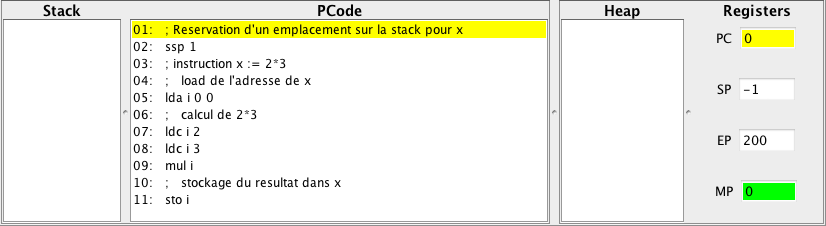
\includegraphics[width=0.9\textwidth]{images/exemple1-step0}
\item Réservation d'un emplacement mémoire sur la stack pour stocker $x$ : \\
            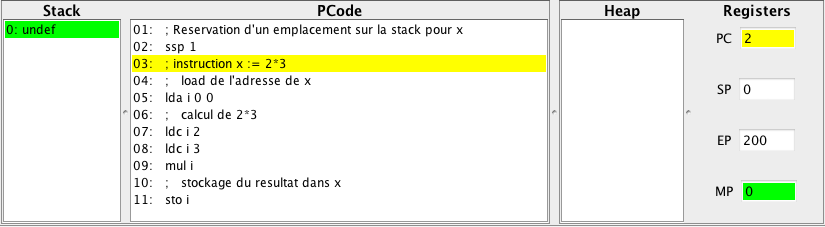
\includegraphics[width=0.9\textwidth]{images/exemple1-step1}
\item Load de l'adresse de $x$ situé en position 0 ($q(x)=0$) du contexte courant (la différence de profondeur $d(x)=0$) : \\
            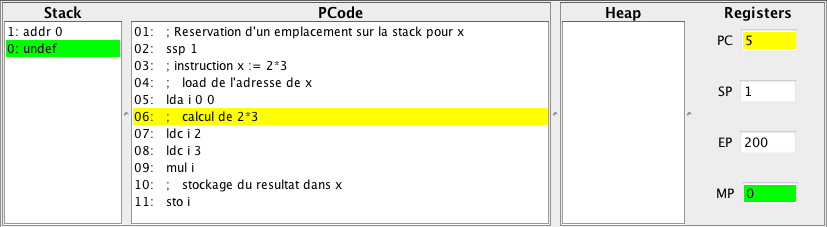
\includegraphics[width=0.9\textwidth]{images/exemple1-step2} 
            \`A noter que si l'on avait voulu accéder depuis une fonction $fct()$ à une variable $a$ déclarée dans la fonction $fctPere()$ parente de $fct()$, la différence de profondeur $d(a)$ aurait été de 1. De même, si $a$ avait été déclarée dans $fctGrandPere()$, $d(a)$  vaudrait 2, etc.
\item Load de la constante entière 2 :\\
            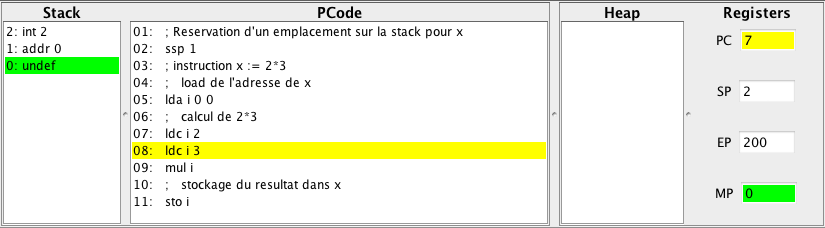
\includegraphics[width=0.9\textwidth]{images/exemple1-step3} 
\item Load de la constante entière 3 :\\
            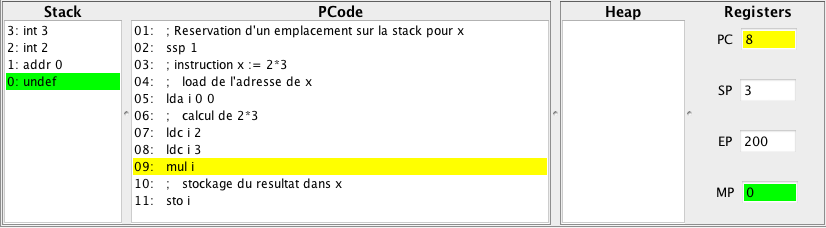
\includegraphics[width=0.9\textwidth]{images/exemple1-step4} 
\item Calcul de la multiplication :\\
            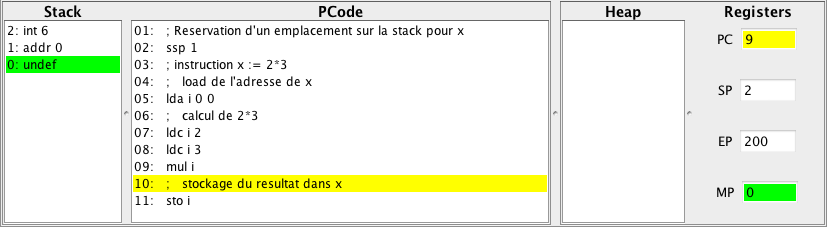
\includegraphics[width=0.9\textwidth]{images/exemple1-step5} 
\item Stockage du résultat dans $x$ :\\
            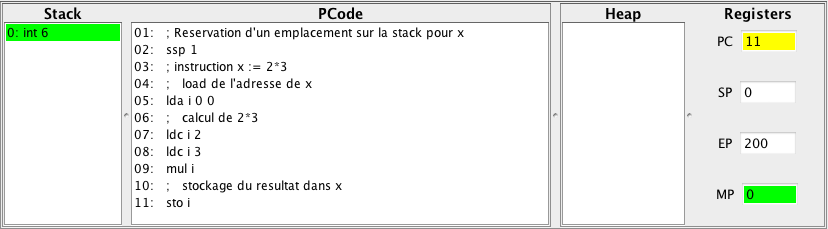
\includegraphics[width=0.9\textwidth]{images/exemple1-step6}             
\end{enumerate}


De la même manière, l'instruction \texttt{y:=3*x+4} avec $x$ et $y$ de type integer sera traduite de la manière suivante :

\begin{tabular}{l}
$PCode(y:=3*x+4)$ \\
\hspace{1cm} $=\ PCode_G(y);\ PCode_D(3*x+4);\ sto\ i $\\
\hspace{1cm} $=\ lda\ i\ d(y)\ q(y);\ PCode_D(3*x+4);\ sto\ i$\\
\hspace{1cm} \vdots\\
\hspace{1cm} $=\ lda\ i\ d(y)\ q(y);\ ldc\ i\ 3;\ lda\ i\ d(x)\ q(x);\ ind\ i;\ mul\ i;\ ldc\ i\ 4;\ add\ i;\ sto\ i $\\
\end{tabular}


\subsection{P-Instructions de branchement}
%%%%%%%%%%%%%%%%%%%%%%%%%%%%%%%%%%%%

\begin{tabular}{|l|l|l|}
\hline
P-Inst                     & Effet                                 & Commentaire\\
\hline
define @k               &                                         & définition d'une étiquette\\
& & \\
ujp @k                    & PC:= adresse(@k)            & branchement inconditionnel\\
& & \\
fjp @k                    & if STORE[SP] = false          & branchement conditionnel\\
                              & then PC := adresse(@k)    &\\
			                  & SP $:=$ SP - 1                  & \\
\hline
\end{tabular}

L'évaluation paresseuse des instructions $and$ et $or$ peut par exemple s'implémenter en utilisant le branchement conditionnel :\\


\begin{tabular}{l}
$PCode(E_1\ or\ E_2)$\\
\hspace{1cm} =  $PCode_D(E_1);$ \\
\hspace{1cm}$\ \ \ \ not  $\\
\hspace{1cm}$\ \ \ \ fjp\ @true$\\
\hspace{1cm}$\ \ \ \ PCode_D(E_2)  $\\
\hspace{1cm}$\ \ \ \ ujp\ @end$\\
\hspace{1cm}$\ \ \ \ define\ @true$\\
\hspace{1cm}$\ \ \ \ ldc\ b\ 1$\\
\hspace{1cm}$\ \ \ \ define\ @end$\\
\end{tabular}
\\

La traduction de l'instruction \texttt{x or false} devient donc en PCode :
\\

\begin{tabular}{l}
$PCode(x or false)$ \\
\hspace{1cm} $=\ PCode_D(x);\ not;\ fjp\ @true;\ PCode_D(true);$\\
\hspace{1cm} $\ \ \ \ ujp\ @end;\ define\ @true;\ ldc\ b\ 1;\ define\ @end$\\
\hspace{1cm} $=\ lda\ i\ d(x)\ q(x);\ ind\ b;\ not\ b;\ fjp\ @true;$\\
\hspace{1cm}$\ \ \ \ \ ldc\ b\ 1;\ ujp\ @end;\ define\ @true;\ ldc\ b\ 1;\ define\ @end$\\
\end{tabular}

Si on exécute ce code dans la GPMachine, on obtient le résultat suivant :
\begin{enumerate}
\item \'{E}tat initial de la machine (après initialisation de la variable $x$) : \\
            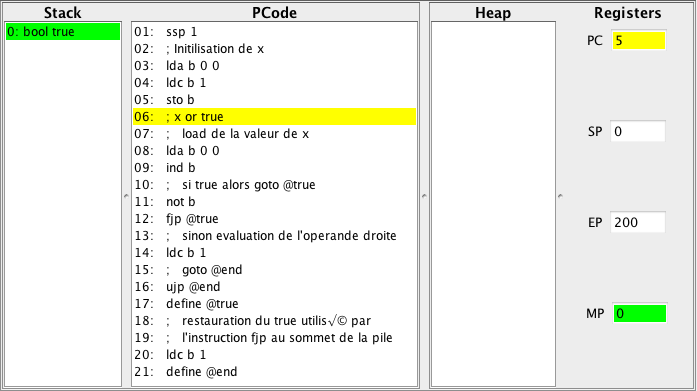
\includegraphics[width=0.9\textwidth]{images/exemple2-step0}
\item Load de l'adresse de la variable $x$ : \\
            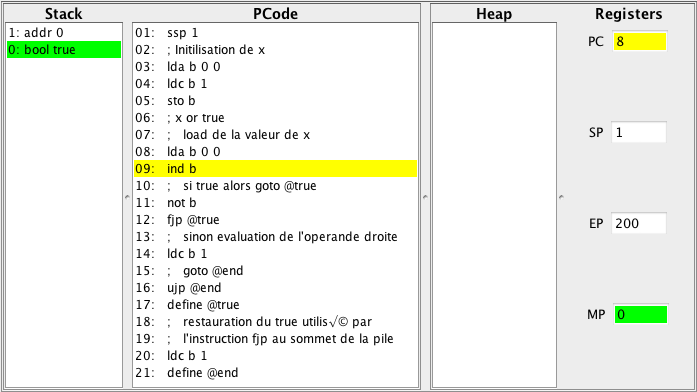
\includegraphics[width=0.9\textwidth]{images/exemple2-step1}
\item Récupération de la valeur stockée à cette adresse : \\
            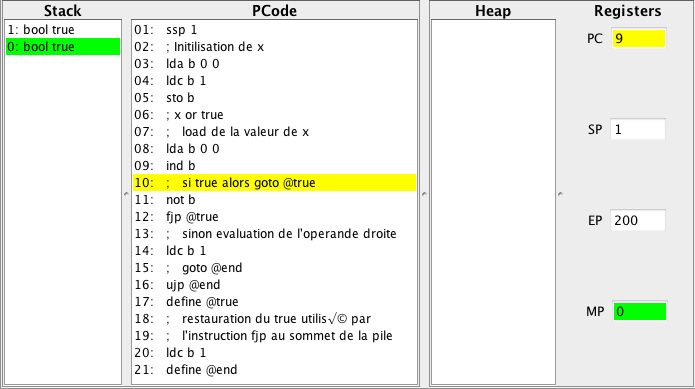
\includegraphics[width=0.9\textwidth]{images/exemple2-step2} 
\item Négation du résultat de l'évaluation de l'expression gauche :\\
            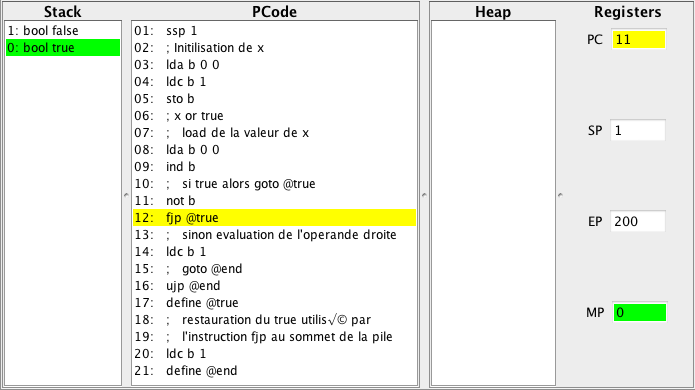
\includegraphics[width=0.9\textwidth]{images/exemple2-step3} 
\item Test sur cette valeur et jump vers le label \texttt{@true} :\\
            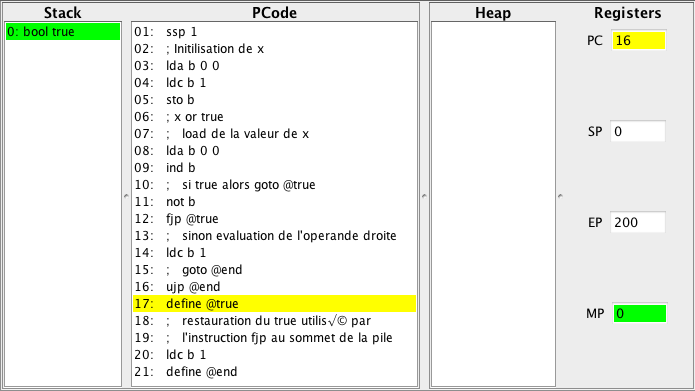
\includegraphics[width=0.9\textwidth]{images/exemple2-step4} 
\item Restauration de la valeur $true$ consommée par l'instruction \texttt{fjp} au sommet de la pile :\\
            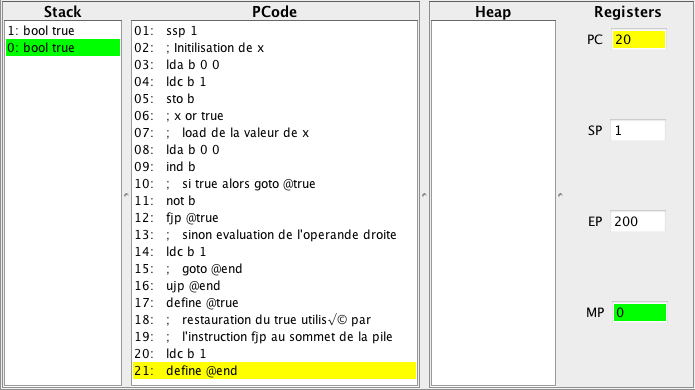
\includegraphics[width=0.9\textwidth]{images/exemple2-step5} 
\end{enumerate}



\subsection{Autres traductions}
%%%%%%%%%%%%%%%%%%%%%%%%%

\begin{tabular}{| l l | l |}
\hline
Fonction                                 &                                                                          & Condition \\
\hline
$PCode(read\ x)=$                  & $PCode_G(x)$                                            & $Type(x)=N$\\
                                                & $ read$                                                      & \\
                                                & $ sto i$                                                      & \\
\hline
$PCode(write\ x)=$                 &  $PCode_D(x) $                                           & $Type(x)=N$\\
                                                & $ prin$                                                      & \\            
\hline
$PCode(if\ E\ then\ I_1\ else\ I_2\ fi) =$ & $PCode_D(E)$                &  $Type(E)=b$\\
                                                                & $fjp\ @else$                                          & \\
                                                                & $PCode(I_1)$                                          & \\
                                                                & $ujp\ @fi$                                 & \\
                                                                & $define\ @else$             &\\
                                                                & $PCode(I_2)$                        & \\
                                                                & $define\ @fi$                                               &\\
\hline
$PCode(while\ E\ do\ I\ od) =$    & $define\ @while$      & $Type(E)=b$\\
                                                    & $PCode_D(E)$            &\\
                                                    & $fjp\ @od $               &\\
                                                    & $PCode(I)$                &\\
                                                    & $ujp\ @while$          &\\
                                                    & $define\ @od$            &\\
\hline
\end{tabular}


\subsection{Traduction d'un programme}
%%%%%%%%%%%%%%%%%%%%%%%%%%%%%%%

\begin{tabular}{| l l | l |}
\hline
Fonction                                 &                                                                          & Condition \\
\hline
$PCode(Program) = $             & $ssp\ s$                                                          & \\
                                              & $ujp\ @begin$                                                 & \\
                                              & $PCode(ProcDeclList) $                                     & \\
                                              & $define\ @begin$                                             & \\
                                              & $PCode(InstList)$                                              & \\ 
                                              & $stp$                                                                 & \\ 
\hline
\end{tabular}

(où ssp s effectue $SP:=MP+s-1$ c-à-d réserve la place dans STORE pour les variables)


\subsection{P-instructions pour les procédures et fonctions}
%%%%%%%%%%%%%%%%%%%%%%%%%%%%%%%%%%%%%%%%%%%%%%%

Les instructions suivantes sont utilisées lors de la définition et l'appel de procédures et fonctions.

\begin{tabular}{|l|l|l|}
\hline
P-Instruction & Signification                            & Commentaire \\
\hline
mst d 	        & STORE[SP+2] := base(d,MP);      & où d = différence profondeur \\
                    &                                                  & appel/déclaration \\
      	            & STORE[SP+3] := MP;         	      & prédécesseur dynamique\\
			        & SP:=SP+5						     	      & réserve l'espace sur la pile pour le bloc \\
			        &                                                  & d'appel\\
\hline
cup p @fct   & MP:=SP-(p+4)						      & réserve l'espace pour les paramètres \\
                    &                                                  & o\`u p = nombre de paramètres\\
			        & STORE[MP+4]:=PC					  & sauver l'adresse de retour\\
			        & PC:=adresse(@k)			              & aller à @fct\\
\hline
ssp s            & SP:=MP+s-1			                      & s = 5 + nombre de cellules mémoire \\
		            &                                                  & pour les paramètres et les variables de la \\
                    &                                                  & fonction/procédure \\
\hline
retp            	& SP:=MP-1							           & libère l'espace occupé\\
		            & PC:=STORE[MP+4]					   & aller à l'instruction qui suit l'appel\\
		            & MP:=STORE[MP+2]					   & registre MP à jour\\
\hline
retf            	& SP:=MP-1							           & libère l'espace occupé\\
                 	& SP:=SP+1							           & réserve une case pour la valeur de retour\\
                 	& STORE[SP]:=STORE[MP]		           & stocke la valeur de retour en haut de la pile\\
		            & PC:=STORE[MP+4]					   & aller à l'instruction qui suit l'appel\\
		            & MP:=STORE[MP+2]					   & registre MP à jour\\		            
\hline
\end{tabular}

Avec base(d,MP) $:=$ if (d=0) then MP else base(d-1,STORE[MP$+$1]) fi  

\subsection{Traduction des procédures, fonctions et paramètres}
%%%%%%%%%%%%%%%%%%%%%%%%%%%%%%%%%%%%%%%%%%%%%%%%%

\subsubsection{PCode pour la déclaration d'une procédure}
%-------------------------------------------------

\begin{tabular}{| l l |}
\hline
Fonction                                 &                                                                         \\
\hline
$PCode(ProcDecl)=$               & $define\ @proc$                                             \\
                                              & $ssp\  s$ \\
                                              & $ujp\  @procBody$                            \\
                                              & $PCode(ProcDeclList)$                                     \\
                                              & $define\ @procBody$\\
                                              & $PCode(InstList)$\\
                                              & $retp$  \\
\hline
\end{tabular}


\subsubsection{PCode pour un appel de procédure}
%-------------------------------------------

\begin{tabular}{| l l |}
\hline
Fonction                                 &                                                                         \\
\hline
$PCode(proc(e_1, e_2, ..., e_n)) =$    & $mst\ d$ \\ 
                                                         & $PCode_A(e_1) $ \\
                                                         & $PCode_A(e_2)$\\
                                                         & $...$\\
                                                         & $PCode_A(e_n)$\\
                                                         & $cup\ p\ @proc$\\
\hline
\end{tabular}
\\

avec

\begin{tabular}{ll}
$PCode_A(e)= PCode_G(e)$  &\ si e est un paramètre passé par adresse\\
$PCode_A(e)= PCode_D(e)$  &\  si e est un paramètre passé par valeur\\
\end{tabular}
\\

$PCode_G$ pour les paramètres

\begin{tabular}{ll}
$PCode_G(x)=\ lda\ T\ d(x)\ q(x)$ & \ si x est une variable locale ou globale de type T\\
$PCode_G(x)= lda\ T\ d(x)\ q(x)$  & \ si x est un paramètre passé par valeur de type T\\
$PCode_G(x)= lod\ a\ d(x)\ q(x)$ & \ si x est un paramètre passé par adresse\\
\end{tabular}

\subsubsection{PCode pour la déclaration d'une fonction}
%-------------------------------------------------

\begin{tabular}{| l l |}
\hline
Fonction                                 &                                                                         \\
\hline
$PCode(ProcDecl)=$               & $define\ @fct$                                             \\
                                              & $ssp\  s$\\
                                              & $ujp\  @fctBody$                            \\
                                              & $PCode(FctDeclList)$                                     \\
                                              & $define\ @fctBody$\\
                                              & $PCode(InstList)$\\
                                              & $retf$  \\
\hline
\end{tabular}
\\

\paragraph{PCode pour une l'instruction return}

Contrairement aux procédures, les fonctions renvoient une valeur à l'appelant. En P-Code, la valeur est placée au sommet de la pile une fois de retour dans le contexte de l'appelant. La valeur retournée est celle située à l'adresse 0 dans le contexte de la fonction appelée. Une instruction \texttt{return} sera donc traduite en PCode de la manière suivante :

\begin{tabular}{| l l | l |}
\hline
Fonction                                 &                                   & Condition \\
\hline
$ PCode(return \  e)=$            & $ lda \ T \ 0 \ 0 $     &  $Type(e)=T$ \\
                                              & $ PCode_{D}(e) $        & \\
                                              & $ sto \ T $                 & \\
                                              & $ retf $                      & \\
\hline
\end{tabular}
\\



\subsubsection{PCode pour un appel de fonction}
%-------------------------------------------

\begin{tabular}{| l l |}
\hline
Fonction                                 &                                                                         \\
\hline
$PCode(fct(e_1, e_2, ..., e_n)) =$       & $mst\ d$ \\ 
                                                         & $PCode_A(e_1)$ \\
                                                         & $PCode_A(e_2)$ \\
                                                         & $...$ \\
                                                         & $PCode_A(e_n)$\\
                                                         & $cup\ p\ @fct$\\
\hline
\end{tabular}


\subsubsection{Bloc d'appel de procédure/fonctions}
%-------------------------------------------

La structure du bloc d'appel d'une procédure ou d'une fonction est présenté dans la figure suivante. Cet espace est réservé sur la pile au moment de l'exécution d'une instruction \texttt{mst}.


\begin{center}
	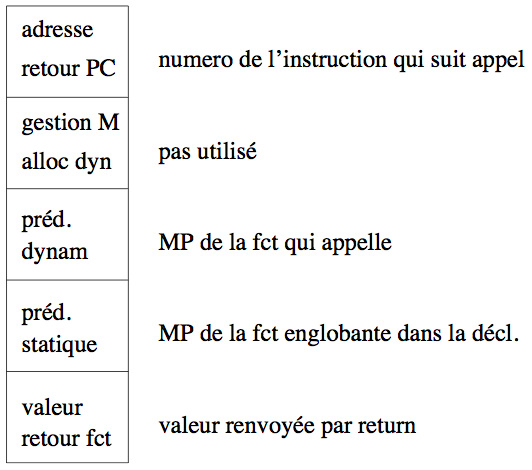
\includegraphics[width=0.5\textwidth]{images/bloc-appel-proc}	
\end{center}
	
	
\subsubsection{Exemple d'appel de fonction}
%-------------------------------------

L'exemple suivant présente un appel de fonction avec passage de paramètres et le renvoi d'une valeur au programme appelant. Sa syntaxe correspond à celle définie dans le cadre du TP compilateur $LSD^{{12}}$.

\lstset{language=lsd12,
breaklines=true,
showstringspaces=false,
frame=single
}
\begin{lstlisting}
program a;
function main():void;
var
	x int;
	function addTo(a : int, b : int):int;
		var
 		begin
			return a + b;
		end;
begin
	x := 2;
	x := addTo(x, 3);
end;
end;
\end{lstlisting}

La traduction en PCode devient alors :

\lstset{language=pcode,
breaklines=true,
showstringspaces=false,
frame=single
}
\begin{lstlisting}
; ************* Start program *************
ssp 1
ujp @begin
; ------ Start function addTo ------
define @addTo
ssp 7
lda i 0 0
lod i 0 5
lod i 0 6
add i
sto i
retf
; ********************
; Start program :
; ********************
define @begin
lda i 0 0
ldc i 2
sto i
lda i 0 0
mst 0
lod i 0 0
ldc i 3
cup 2 @addTo
sto i
stp
\end{lstlisting}


\subsection{Utilisation du tas (heap)}
%%%%%%%%%%%%%%%%%%%%%%%%%%%%

\begin{tabular}{|l|l|c|c|}
\hline
P-Inst                     & Signification                                   & Condition      & Résultat \\
\hline
new                       & if (EP-STORE[SP] $\leq$ SP)              & (i)                  & (a) \\
                             & then error(``Heap Overflow'')           &                     & \\
                             & else                                                  &                     & \\
                             & \hspace{1cm}EP $:=$EP-STORE[SP]; &                     & \\
                             & \hspace{1cm}STORE[SP] $:=$ EP+1; &                     & \\
                             & fi;                                                     &                     & \\
\hline
\end{tabular}

Attention, il n'y a pas d'instruction $free$ disponible en P-Code.

\subsubsection{Exemple d'utilisation du tas}
%-------------------------------------

Le PCode suivant réserve 4 emplacements sur le $heap$ et les initialise avec les valeurs 1, 2, 3 et 4.

\lstset{language=pcode,
breaklines=true,
showstringspaces=false,
frame=single
}
\begin{lstlisting}
ssp 1
; Reservation de 4 blocs dans le heap
lda a 0 0
ldc i 4
new
; bloc[0] := 1
lda a 0 0
ind a
ldc i 1
sto i
; bloc[1] := 2
lda a 0 0
ind a
ldc a 1
add a
ldc i 2
sto i
; bloc[2] := 3
lda a 0 0
ind a
ldc a 2
add a
ldc i 3
sto i
; bloc[3] := 4
lda a 0 0
ind a
ldc a 3
add a
ldc i 4
sto i
stp
\end{lstlisting}

Si on exécute ce code dans la GPMachine, on obtient le résultat suivant :
\begin{enumerate}
\item Passage des valeurs nécessaires à l'instruction \texttt{new} au sommet de la pile. \texttt{STORE[1]} contient l'adresse de la cellule mémoire dans laquelle l'adresse du premier bloc réservé sera placée. \texttt{STORE[2]} contient le nombre de cellules mémoires à réserver.  \\
            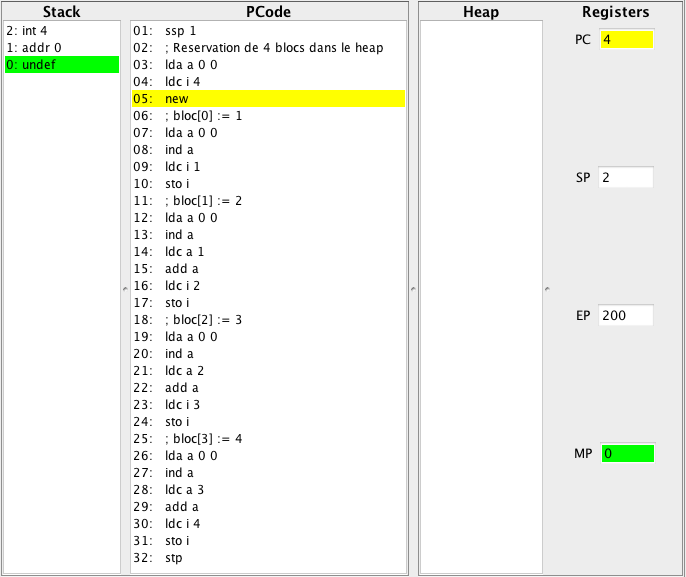
\includegraphics[width=0.9\textwidth]{images/exemple-heap-0}
\item Exécution de l'instruction \texttt{new} : \\
            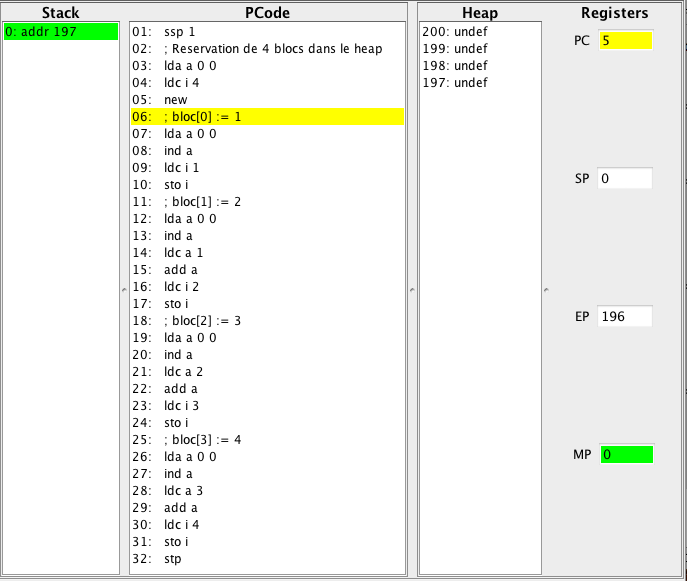
\includegraphics[width=0.9\textwidth]{images/exemple-heap-1}
\item Initialisation des cellules mémoires réservées sur le $heap$ : \\
            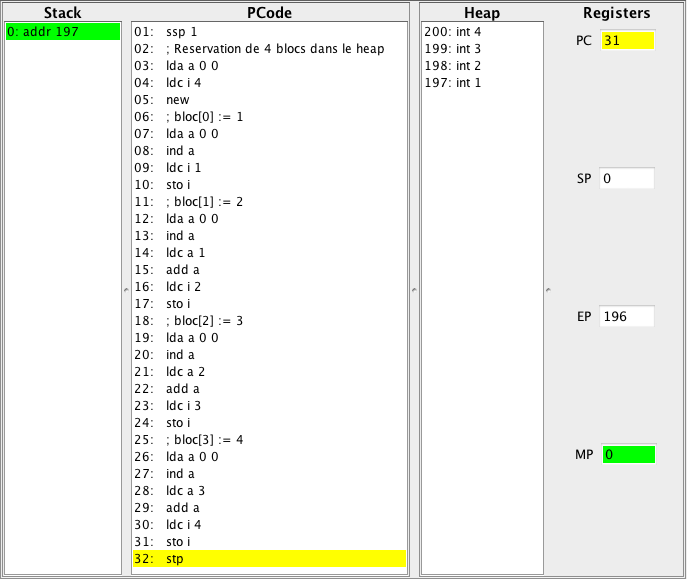
\includegraphics[width=0.9\textwidth]{images/exemple-heap-2} 
\end{enumerate}

\end{document}
%%%%%%%%%%%%%%%%%%%%%%%%%%%%%%%%%%%%%%%%%%%%%%%%%%%%%%%%%%%%%%%%%%%%%%%%%%%%%%%%%%%%%%